%   Filename    : chapter_4.tex 
\chapter{Results}

\section{Dataset}
We have built a balanced dataset containing a total of 3206 new articles (1603 real and fake news) named Filipion Fake News 2024. This dataset is combined with Filipino Fake News dataset for training purposes. Figures \ref{fig:oov_data} to \ref{fig:sw_data} depicts the average OOV count, average readability index, and average stop words count of the two datasets. Filipino Fake News 2024 has an average OOV count, readability index, and stop words count of 22.2, 19.7, and 74.5 respectively. On the other hand, in the same order of values, Filipino Fake News has 17.6, 20.5, and 77.8 respectively. This shows that on average, news articles in Filipino Fake News is more readable, has lower OOV count, and higher Stop words count.

\begin{figure}[h!]
    \centering
    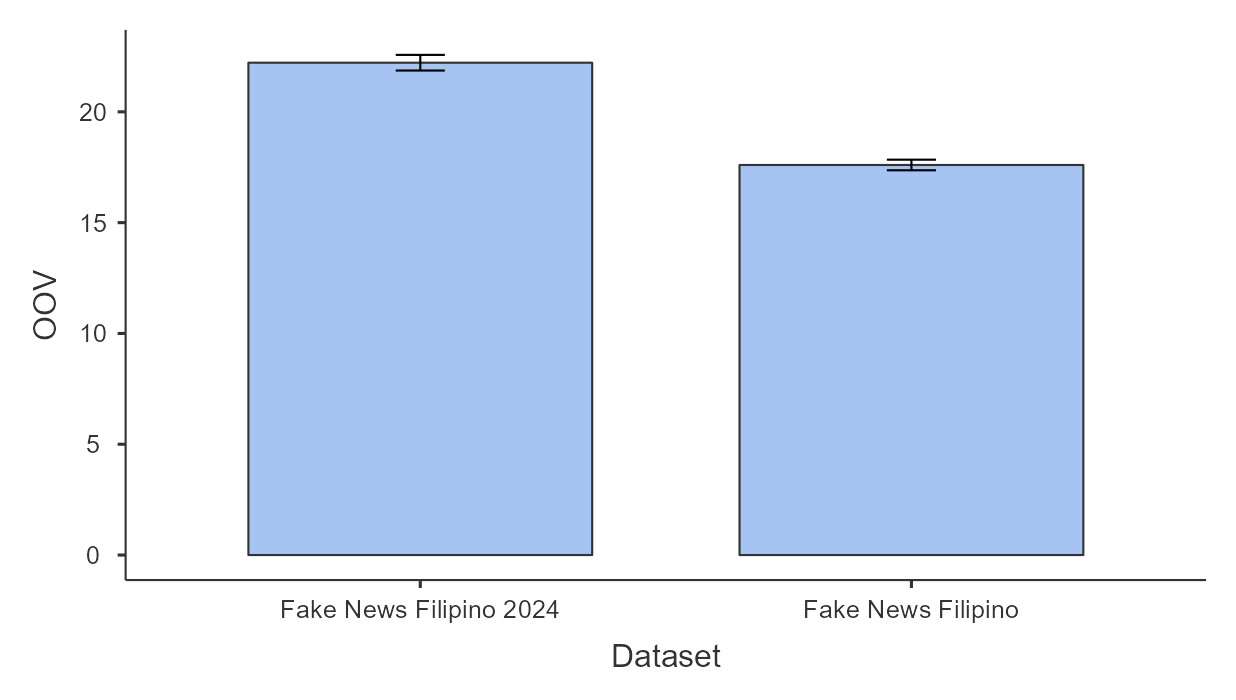
\includegraphics[width=\textwidth,height=\textheight, keepaspectratio]{figures/stats/oov_data.png}
        \caption{OOV count Bar Plot of Filipino Fake News and Filipino Fake News 2024}
        \label{fig:oov_data}
\end{figure}
\begin{figure}[h!]
    \centering
    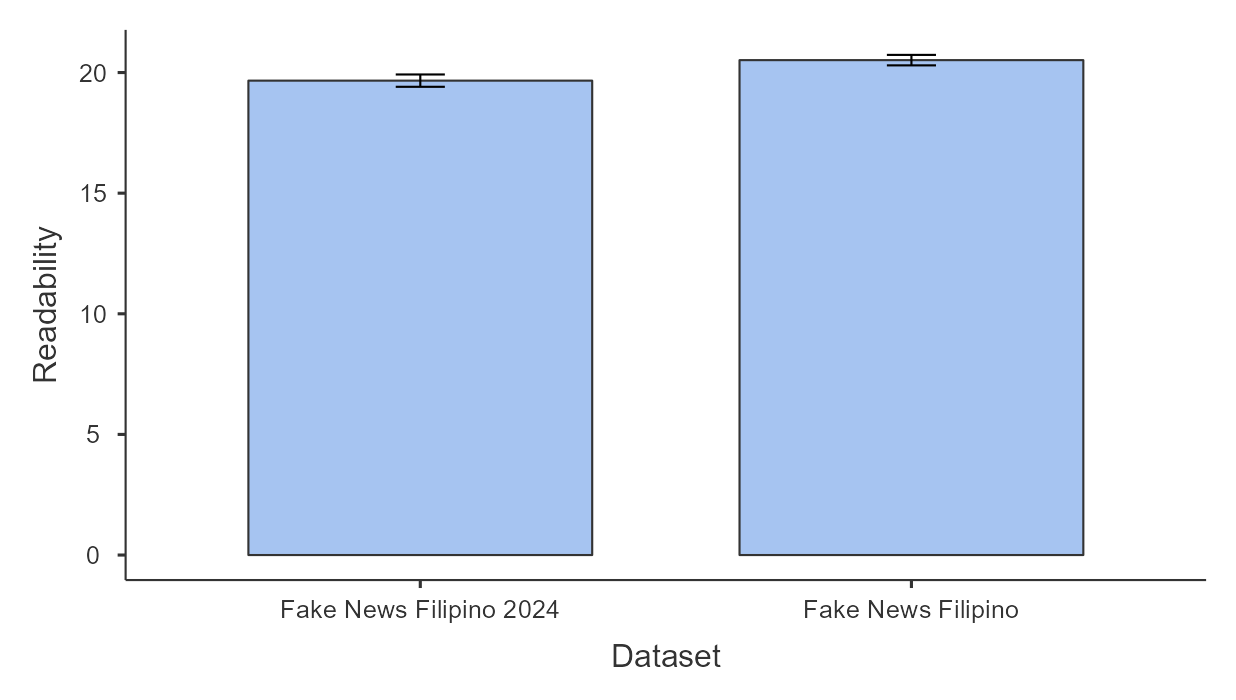
\includegraphics[width=\textwidth,height=\textheight, keepaspectratio]{figures/stats/read_data.png}
        \caption{Readability Index Bar Plot of Filipino Fake News and Filipino Fake News 2024}
        \label{fig:read_data}
\end{figure}
\begin{figure}[h!]
    \centering
    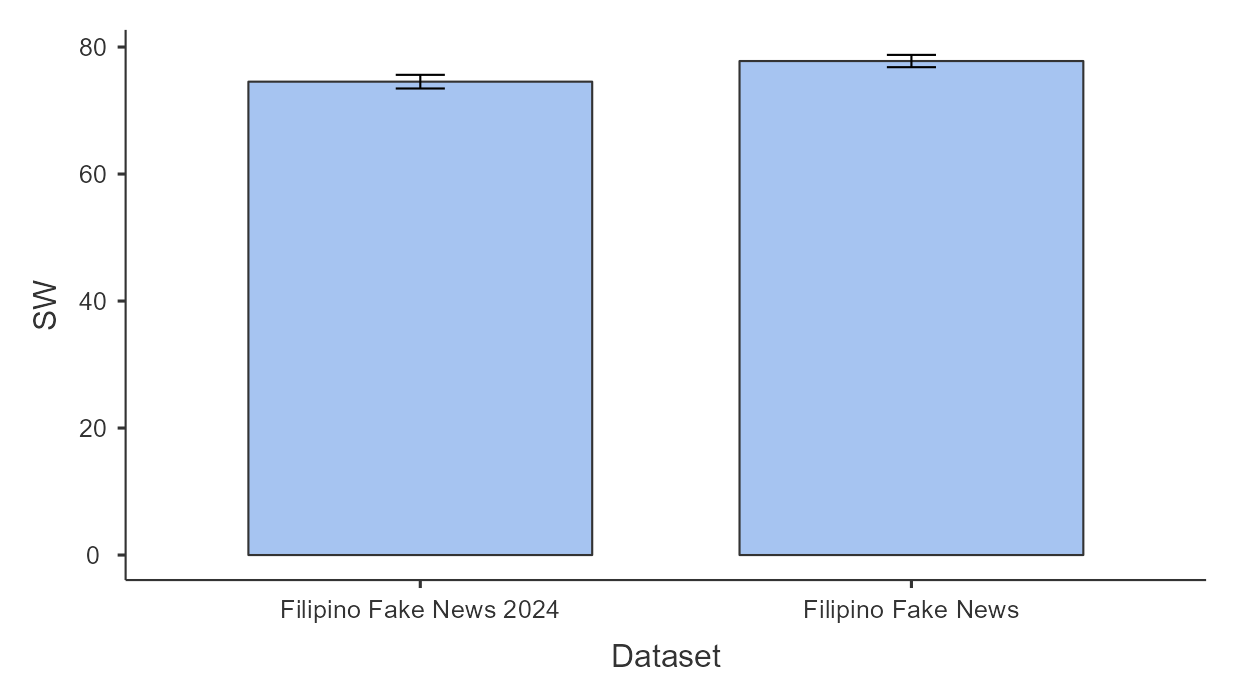
\includegraphics[width=\textwidth,height=\textheight, keepaspectratio]{figures/stats/sw_data.png}
        \caption{Stop Words Bar Plot of Filipino Fake News and Filipino Fake News 2024}
        \label{fig:sw_data}
\end{figure}

\section{Classifiers without Hyperparameter Tuning}

The models were trained on the combined dataset without hyperparameter tuning.

Figure \ref{MNB_default} shows the confusion matrix of \textbf{Multinomial Naive Bayes} without grid search. The model did not misclassify any instance of real news as fake news. However, it misclassified 537 instances of fake news as real news, significantly lowering its recall for fake news. It yielded an accuracy of approximately 0.58. It had the lowest recall for fake news at 0.16, signifying difficulty in identify true instances of fake news and a high false positive rate. The F1-score of real news and fake news were 0.70 and 0.28 respectively. These were relatively low scores. 

\begin{figure}[h!]
    \centering
    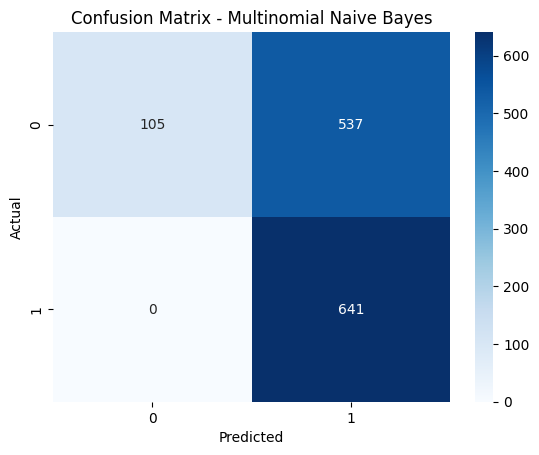
\includegraphics[width=0.6\textwidth,height=0.6\textheight, keepaspectratio]{figures/hyperparam/MNB_default.png}
        \caption{Confusion Matrix of Multinomial Naive Bayes without Grid Search}
        \label{MNB_default}
\end{figure}

As shown in the confusion matrix of \textbf{Logistic Regression} at Figure \ref{LR_default}, the model misclassified 42 instances of fake news as real news and 51 instances of real news as fake news. It yielded an accuracy of approximately 0.93. It had a high recall for real news and fake news at both 0.93 and 0.92 respectively. The f1-scores for both real news and fake news were 0.93.

\begin{figure}[h!]
    \centering
    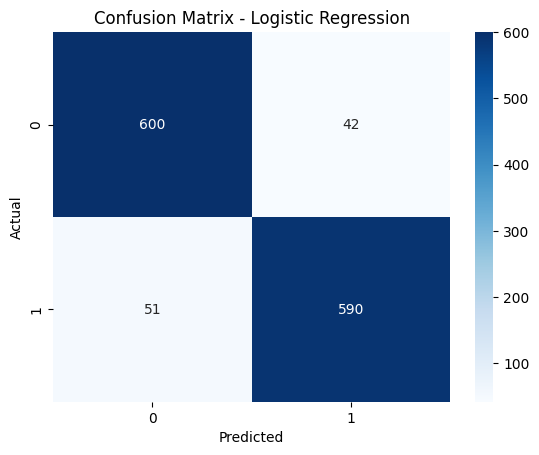
\includegraphics[width=0.6\textwidth,height=0.6\textheight, keepaspectratio]{figures/hyperparam/LR_default.png}
        \caption{Confusion Matrix of Logistic Regression without Grid Search}
        \label{LR_default}
\end{figure}

Figure \ref{RF_default} depicts the confusion matrix of \textbf{Random Forest}. The model misclassified 66 instances of fake news and 59 instances of real news. It yielded an accuracy of approximately 0.90. It had a recall of 0.90 and 0.91 for fake news and real news respectively. The f1-score of both classes was 0.90, implying balanced metrics.

\begin{figure}[h!]
    \centering
    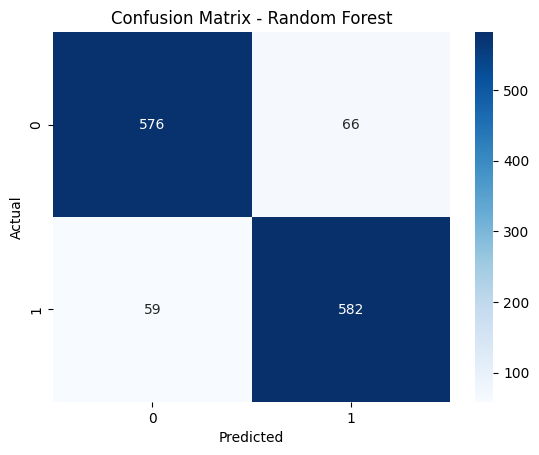
\includegraphics[width=0.6\textwidth,height=0.6\textheight, keepaspectratio]{figures/hyperparam/RF_default.png}
        \caption{Confusion Matrix of Multinomial Naive Bayes without Grid Search}
        \label{RF_default}
\end{figure}

Based on Figure \ref{SVC_default}, \textbf{Support Vector Classifier}, misclassified 169 instances of fake news and 70 instances of real news. It had an accuracy of approximately 0.81. It had a relatively lower recall for fake news at 0.74. The f1-scores for real news and fake news were 0.80 and 0.83 respectively. 

\begin{figure}[h!]
    \centering
    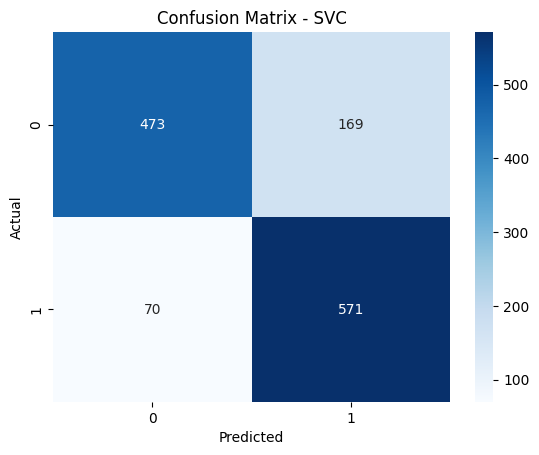
\includegraphics[width=0.6\textwidth,height=0.6\textheight, keepaspectratio]{figures/hyperparam/SVC_default.png}
        \caption{Confusion Matrix of Multinomial Naive Bayes without Grid Search}
        \label{SVC_default}
\end{figure}

Results without hyperparameter tuning are summarized in Table \ref{tab:no_hyperparam_summary}. As shown in Table \ref{tab:no_hyperparam_summary}, Logistic Regression had the highest f1-scores while Multinomial Naive Bayes scored the lowest.

\begin{table}[ht]
    \centering
    \begin{tabular}{|l|ccc|ccc|}
    \hline
    & \multicolumn{3}{c|}{Multinomial Naive Bayes} & \multicolumn{3}{c|}{Logistic Regression} \\
    \hline
    & Precision & Recall & F1-Score & Precision & Recall & F1-Score \\
    \hline
    Fake & 1.00 & 0.16 & 0.28 & 0.92 & 0.93 & 0.93 \\
    Not Fake & 0.54 & 1.00 & 0.70 & 0.93 & 0.92 & 0.93 \\
    Accuracy & & & 0.58 & & & 0.93 \\
    \hline
    & \multicolumn{3}{c|}{Random Forest} & \multicolumn{3}{c|}{Support Vector Classifier} \\
    \hline
    & Precision & Recall & F1-Score & Precision & Recall & F1-Score \\
    \hline
    Fake & 0.91 & 0.90 & 0.90 & 0.87 & 0.74 & 0.80 \\
    Not Fake & 0.90 & 0.91 & 0.90 & 0.77 & 0.89 & 0.83 \\
    Accuracy & & & 0.90 & & & 0.81 \\
    \hline
    \end{tabular}
    \caption{Performance Metrics for Classifiers with Hyperparameter Tuning}
    \label{tab:no_hyperparam_summary}
\end{table}



\section{Classifiers with Hyperparameter Tuning}
\label{sec:ParamTuning}
To the determine the optimal hyperparameters, all models were trained and tested on the combined dataset using grid search with five-fold cross validation.

Figure \ref{MNB_hyperparam} shows the performance of \textbf{Multinomial Naive Bayes} with an alpha of 0.01, the optimal hyperparameter based on the cross validation. The model misclassified 155 instances of fake news and 18 instances of real news. It yielded an accuracy of approximately 0.865. It had the lowest recall for fake news at 0.87.

\begin{figure}[h!]
\centering
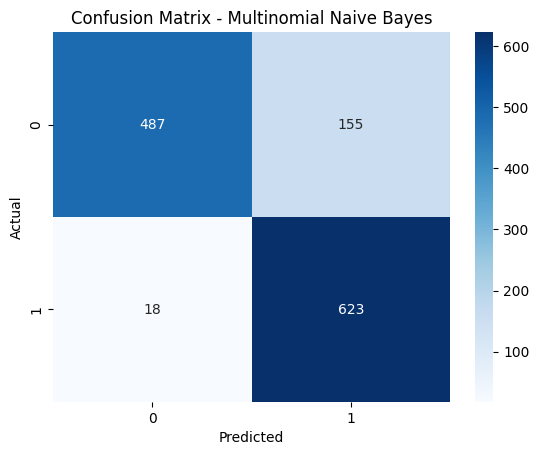
\includegraphics[width=0.6\textwidth,height=0.6\textheight, keepaspectratio]{figures/hyperparam/MNB.png}
    \caption{Confusion Matrix of Multinomial Naive Bayes with alpha = 0.01}
    \label{MNB_hyperparam}
\end{figure}

The best hyperparameter for \textbf{Logistic Regression} was max\_iter = 2000. As shown in Figure \ref{LR_hyperparam}, Logistic Regression misclassified 42 instances of fake news and 51 instances of real news. It yielded an accuracy of 0.928 and an f1-score of 0.93 for both real news and fake news. 

\begin{figure}[h!]
\centering
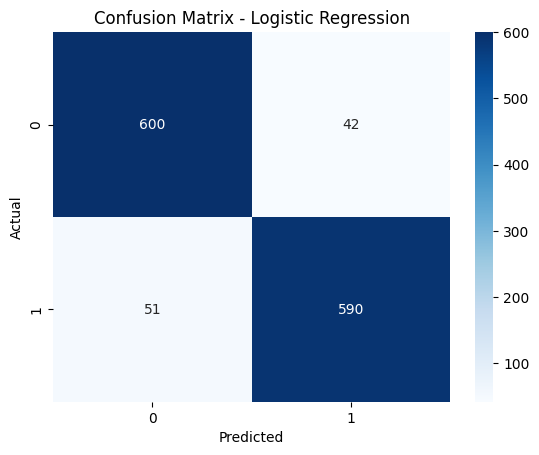
\includegraphics[width=0.6\textwidth,height=0.6\textheight, keepaspectratio]{figures/hyperparam/LR.png}
    \caption{Confusion Matrix of Linear Regression with max\_iter = 2000}
    \label{LR_hyperparam}
\end{figure}

For \textbf{Random Forest}, max\_depth = 20 was the optimal hyperparameter. The performance of Random Forest is shown in Figure \ref{RF_hyperparam}. The model misclassified 80 instances of fake news and 63 instances of real news. It yielded an accuracy of 0.889 with an f1-score of 0.89 for both fake news and real news.

\begin{figure}[h!]
\centering
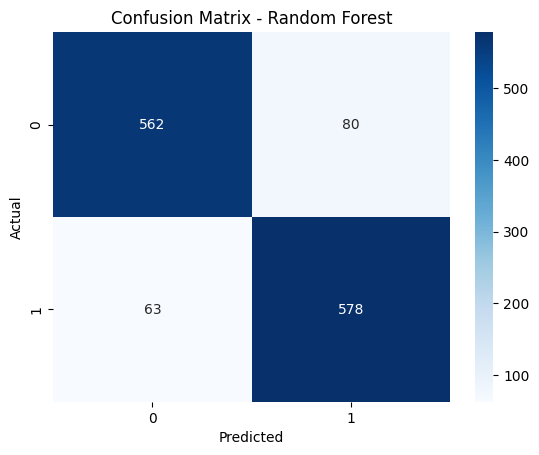
\includegraphics[width=0.6\textwidth,height=0.6\textheight, keepaspectratio]{figures/hyperparam/RF.png}
    \caption{Confusion Matrix of Random Forest with max\_depth = 20}
    \label{RF_hyperparam}
\end{figure}

For \textbf{Support Vector Classifier}, the optimal hyperparameter was C = 0.1 with a linear kernel. As shown in Figure \ref{SVC_hyperparam}, the model misclassified 42 instances of fake news and 51 instances of real news. It yielded an accuracy of 0.928 and an f1-score of 0.93 for both fake news and real news.

Both Support Vector Classifier and Logistic Regression yielded the highest accuracy with hyperparameter tuning.

\begin{figure}[h!]
\centering
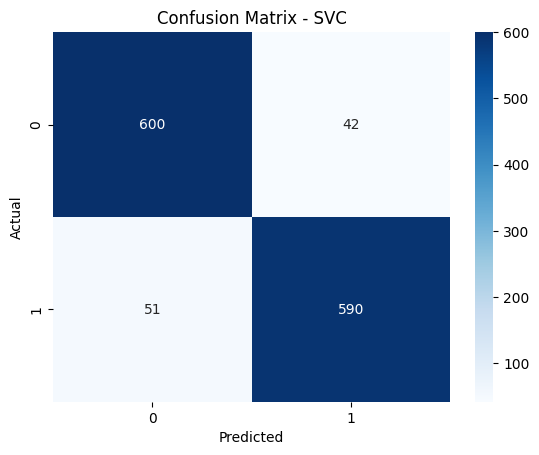
\includegraphics[width=0.6\textwidth,height=0.6\textheight, keepaspectratio]{figures/hyperparam/SVC.png}
    \caption{Confusion Support Vector Classifier with a linear kernel and C = 0.1}
    \label{SVC_hyperparam}
\end{figure}

The results are summarized in Table \ref{tab:hyperparam_summary}. Both Logistic Regression and Support Vector Classifier scored the highest f1-scores while Random Forest scored the lowest. Comparing the accuracies of the classifiers without hyperparameter tuning in Table \ref{tab:no_hyperparam_summary} and their accuracies with hyperparameter tuning in Table \ref{tab:hyperparam_summary}, hyperparameter tuning significantly increased the accuracy of Multinomial Naive Bayes and Support Vector Classifier. However, hyperparameter tuning did not have any significant impact on the accuracies of Logistic Regression and Random Forest.

\begin{table}[ht]
    \centering
    \begin{tabular}{|l|ccc|ccc|}
    \hline
    & \multicolumn{3}{c|}{Multinomial Naive Bayes} & \multicolumn{3}{c|}{Logistic Regression} \\
    \hline
    & Precision & Recall & F1-Score & Precision & Recall & F1-Score \\
    \hline
    Fake & 0.93 & 0.76 & 0.85 & 0.92 & 0.93 & 0.93 \\
    Not Fake & 0.80 & 0.97 & 0.88 & 0.93 & 0.92 & 0.93 \\
    Accuracy & & & 0.87 & & & 0.93 \\
    \hline
    & \multicolumn{3}{c|}{Random Forest} & \multicolumn{3}{c|}{Support Vector Classifier} \\
    \hline
    & Precision & Recall & F1-Score & Precision & Recall & F1-Score \\
    \hline
    Fake & 0.90 & 0.88 & 0.89 & 0.92 & 0.93 & 0.93 \\
    Not Fake & 0.88 & 0.90 & 0.89 & 0.93 & 0.92 & 0.93 \\
    Accuracy & & & 0.89 & & & 0.93 \\
    \hline
    \end{tabular}
    \caption{Performance Metrics for Classifiers with Hyperparameter Tuning}
    \label{tab:hyperparam_summary}
\end{table}
    
\section{Accuracy Testing}

Using the optimal hyperparameters in Section \ref{sec:ParamTuning}, all four models were trained and tested using five-fold cross validation six times, a total of 30 tests, across three datasets: Fake News Filipino (2020), Fake News Filipino 2024 (2024), and the combined corpus with the two datasets. Average accuracies of the models are shown in Table \ref{tab::AverageAccuracies}. Logistic Regression and Support Vector Classifier scored the highest average accuracy in both Fake News Filipino and Fake News Filipino 2024. But for the combined dataset, only Logistic Regression yielded the highest average accuracy. Compared to the other models across the three datasets, Multinomial Naive Bayes and Random Forest performed relatively worst in the combined dataset with accuracies of 86.0\% and 88.8\% respectively. Table \ref{tab::AverageAccuracies} shows the average accuracies of the models. The box plot of the accuracies is depicted in Figure \ref{fig:box_plot_accuracy}.

\begin{tabularx}{\textwidth}{|l|l|c|}
    \hline Classifier & Dataset & Average Accuracy \\ \hline
    \endfirsthead

    \hline
    \multicolumn{3}{|r|}
    {Continued from previous page.} \\
    \hline
    Classifier  & Dataset & Average Accuracy \\ \hline
    \endhead

    \hline \multicolumn{3}{|r|}{{Continued on next page...}} \\ \hline
    \endfoot
    
    \hline
    \caption{Average Accuracies}
    \endlastfoot

    Logistic Regression & Fake News Filipino & 0.951 \\
    & Fake News Filipino 2024 & 0.947\\
    & Combined & 0.924 \\
    \hline
    Multinomial Naive Bayes & Fake News Filipino & 0.923 \\
    & Fake News Filipino 2024 & 0.885 \\
    & Combined & 0.860 \\
    \hline
    Random Forest & Fake News Filipino & 0.919 \\
    & Fake News Filipino 2024 & 0.926 \\
    & Combined & 0.888 \\  
    \hline
    Support Vector Classifier & Fake News Filipino & 0.951 \\
    & Fake News Filipino 2024 & 0.947 \\
    & Combined & 0.922
\label{tab::AverageAccuracies}
\end{tabularx}

\begin{figure}[h!]
    \centering
    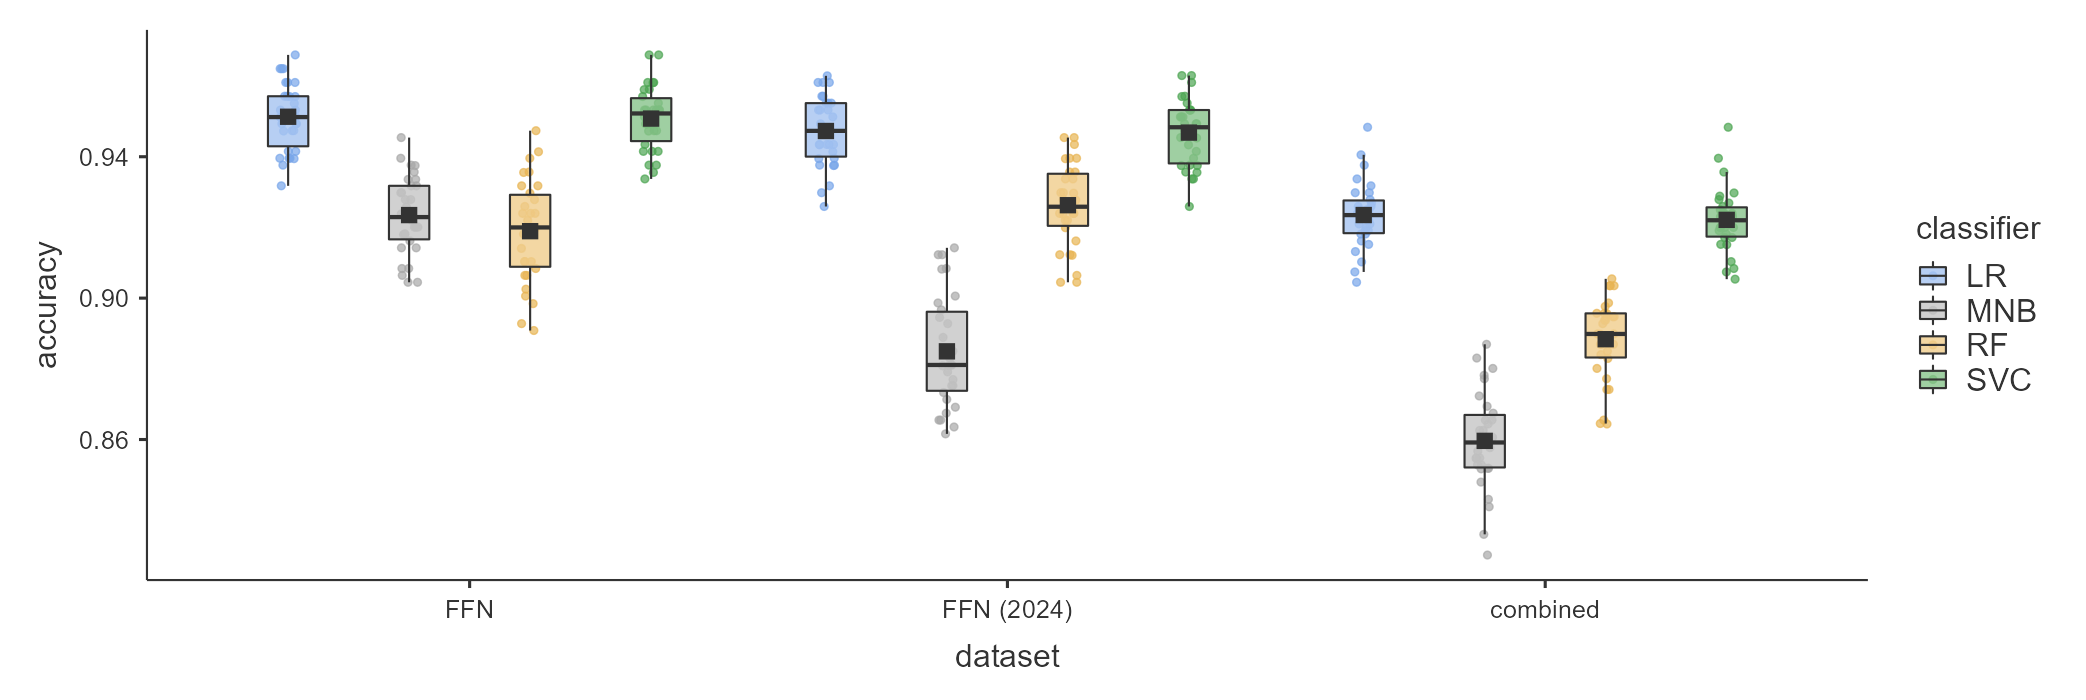
\includegraphics[width=\textwidth,height=\textheight, keepaspectratio]{figures/stats/box_plot.png}
        \caption{Box plot of the accuracies accross datasets}
        \label{fig:box_plot_accuracy}
\end{figure}

The Shapiro-Wilk Test of Normality was used to assess the normality of each group in a two-way format, where accuracies were the dependent variable, and datasets and classifiers were the factors. As shown in Table \ref{tab::normality_tests}, all groups have p-values greater than or equal to 0.05 indicating that the data is normally distributed in the two-way format. However, with a p-value (0.003) lower than 0.05, Levene's Homogeneity Test determined the variances of the groups to be heterogenous.

\begin{tabularx}{\textwidth}{|l|l|l|l|}
    \hline
    Dataset & Classfier & Statistic & p-value \\
    \hline
    Fake News Filipino & LR & 0.968 & 0.492 \\
    & MNB & 0.971 & 0.571 \\
    & RF & 0.985 & 0.938 \\
    & SVC & 0.972 & 0.603 \\
    \hline
    Fake News Filipino 2024 & LR & 0.963 & 0.363 \\
    & MNB & 0.940 & 0.928 \\
    & RF & 0.962 & 0.342 \\
    & SVC & 0.972 & 0.598 \\
    \hline
    Combined & LR & 0.979 & 0.793 \\
    & MNB & 0.981 & 0.852 \\
    & RF & 0.934 & 0.063 \\
    & SVC & 0.950 & 0.164 \\
    \hline
\caption{Shapiro-Wilk normality test}
\label{tab::normality_tests}
\end{tabularx}

To determine if there were significant differences between accuracies of different classifiers in different datasets, and taking into account the heteroscedacity of the data, two-way ANOVA for trimmed means was performed. As shown in Table \ref{tab::two-way} there was a significant difference (p-value = 0.001) between accuracies in different datasets averaged across the classifiers. Additionally, there was a significant difference (p-value = 0.001) between accuracies in the classifiers averaged across the datasets. Furthermore, their interaction effect was also significant (p-value = 0.001). Thus, accuracy was affected both by the main effects of the dataset and classifier and also their combinations.

\begin{tabularx}{\textwidth}{|l|l|l|}
    \hline
    Factor & Statistic & p-value \\
    \hline
    dataset & 689.45 & 0.001 \\
    \hline
    classifier & 1010.0371 & 0.001 \\
    \hline
    dataset*classifier & 129.07 & 0.001 \\
    \hline
\caption{Two-way ANOVA for Trimmed Means}
\label{tab::two-way}
\end{tabularx}

To determine which classifiers had significant differences within the different datsets, post-hoc mean-separation testing was conducted using Bonferroni Correction for subgroups of each dataset level. As shown in Table \ref{tab::post-hoc-dataset-lvl}, the only subgroups that did not have significant differences were Logistic Regression and Support Vector Classifier across all datasets, as well as Multinomial Naive Bayes and Random Forest in the Fake News Filipino dataset.

The results were reflected in the interaction plot of the accuracies in Figure \ref{fig:interaction_plot}. As shown in Figure \ref{fig:interaction_plot}, the accuracies of Logistic Regression and Support Vector Classifier were almost equal across all datasets. The same could be said for the accuracy of Multinomial Naive Bayes and Random Forest in the Fake News Filipino dataset. It can also be observed that the performance of the classifiers changes depending on the dataset just as the two-way ANOVA suggested.

To determine which classifiers have significant differences between datasets, a similar post-hoc test was conducted for subgroups of each classifier level. Table \ref{tab::post-hoc-classifier-lvl} shows that only Multinomial Naive Bayes has a significant change in performance between Fake News Filipino 2024 and Fake News Filipino dataset. Furthermore, all accuracies of the classfiers differ significantly in the combined dataset compared with their accuracy in either Filipino Fake news or Filipino Fake news 2024.

\begin{figure}[h!]
    \centering
    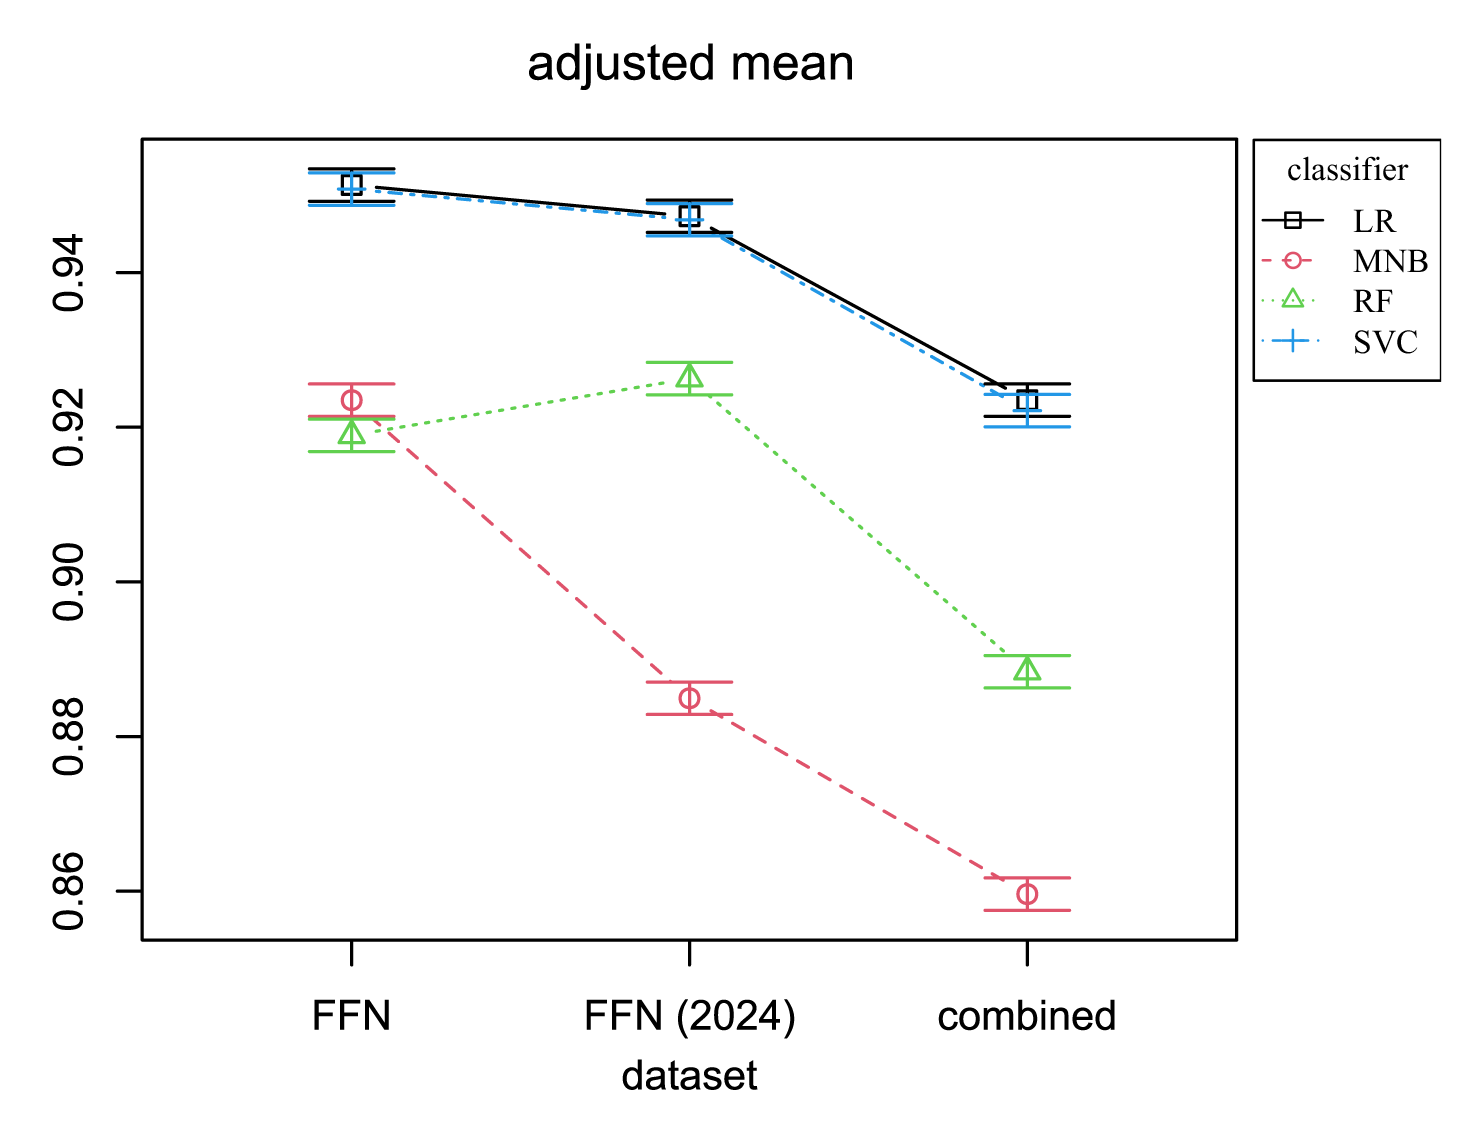
\includegraphics[width=\textwidth,height=\textheight, keepaspectratio]{figures/stats/im.png}
        \caption{interaction plot of accuracies across datasets}
        \label{fig:interaction_plot}
\end{figure}

\begin{tabularx}{\textwidth}{|l|l|l|l|}
    \hline Dataset & Classifier (a) & Classifier(b) & p-value \\ \hline
    \endfirsthead

    \hline
    \multicolumn{4}{|r|}
    {Continued from previous page.} \\

    \hline
    Dataset & Classifier (a) & Classifier(b) & p-value \\ \hline
    \endhead

    \hline \multicolumn{4}{|r|}{{Continued on next page...}} \\ \hline
    \endfoot
    
    \hline
    \caption{Bonferroni correction for subgroups of each dataset level}
    \endlastfoot

    Fake News Filipino & LR & MNB & \textless 0.001 \\
    \cline{3-4}
    & & RF & \textless 0.001 \\
    \cline{3-4}
    & & SVC & 1.00 \\
    \cline{2-4}
    & MNB & RF & 1.00 \\
    \cline{3-4}
    & & SVC & \textless 0.001 \\
    \cline{2-4}
    & RF & SVC &  \textless 0.001 \\
    \hline
    Fake News Filipino 2024 & LR & MNB & \textless 0.001 \\
    \cline{3-4}
    & & RF & \textless 0.001 \\
    \cline{3-4}
    & & SVC & 1.00 \\
    \cline{2-4}
    & MNB & RF & \textless 0.001 \\
    \cline{3-4}
    & & SVC & \textless 0.001 \\
    \cline{2-4}
    & RF & SVC &  \textless 0.001 \\
    \hline
    Combined & LR & MNB & \textless 0.001 \\
    \cline{3-4}
    & & RF & \textless 0.001 \\
    \cline{3-4}
    & & SVC & 1.00 \\
    \cline{2-4}
    & MNB & RF & \textless 0.001 \\
    \cline{3-4}
    & & SVC & \textless 0.001 \\
    \cline{2-4}
    & RF & SVC &  \textless 0.001
\label{tab::post-hoc-dataset-lvl}
\end{tabularx}

\begin{tabularx}{\textwidth}{|l|l|l|l|}
    \hline Classifier & Dataset(a) & Dataset(b) & p-value \\ \hline
    \endfirsthead

    \hline
    \multicolumn{4}{|r|}
    {Continued from previous page.} \\

    \hline
    Classifier & Dataset(a) & Dataset(b) & p-value \\ \hline
    \endhead

    \hline \multicolumn{4}{|r|}{{Continued on next page...}} \\ \hline
    \endfoot
    
    \hline
    \caption{Bonferroni correction for subgroups of each classifier level}
    \endlastfoot

    LR & Fake News Filipino & Fake News Filipino 2024 & 0.485 \\
    \cline{3-4}
    & & Combined & \textless 0.001 \\
    \cline{2-4}
    & Fake News Filipino 2024 & Combined & \textless 0.001 \\
    \hline
    MNB & Fake News Filipino & Fake News Filipino 2024 & \textless 0.001 \\
    \cline{3-4}
    & & Combined & \textless 0.001 \\
    \cline{2-4}
    & Fake News Filipino 2024 & Combined & \textless 0.001 \\
    \hline
    RF & Fake News Filipino & Fake News Filipino 2024 & 0.150 \\
    \cline{3-4}
    & & Combined & \textless 0.001 \\
    \cline{2-4}
    & Fake News Filipino 2024 & Combined & \textless 0.001 \\
    \hline
    SVC & Fake News Filipino & Fake News Filipino 2024 & 0.421 \\
    \cline{3-4}
    & & Combined & \textless 0.001 \\
    \cline{2-4}
    & Fake News Filipino 2024 & Combined & \textless 0.001
\label{tab::post-hoc-classifier-lvl}
\end{tabularx}